\documentclass[fleqn]{article}
\usepackage[margin=1.5cm]{geometry}   % shrink margins
\usepackage{amsmath}    % math equation environments
% \usepackage{amssymb}    % math symbols such as natural numbers N.

% \usepackage{multicol}	% can be used to put enumerate in columns. Usage: \begin{multicols}{NumCols}\begin{enumerate}...

% \newcommand\Item[1][]{ % custom \Item command for block math
%   \abovedisplayskip=0pt\abovedisplayshortskip=0pt~\vspace*{-\baselineskip}}
%   \ifx\relax#1\relax  \item \else \item[#1] \fi

\newcommand*{\perm}[2]{{}^{#1}\!P_{#2}}
\newcommand*{\comb}[2]{{}^{#1}C_{#2}}

\usepackage{tikz}	% for diagrams
\usetikzlibrary{positioning}

% \usepackage{adjustbox}	% align enumerations containing tall objects to top. Usage: \item\adjustbox{valign=t}{...}

% \usepackage{centernot}	% centers not symbol. Usage: \centernot{...}

% Math mode in tables. Usage: use column type C
% \usepackage{array}   % for \newcolumntype macro
% \newcolumntype{C}{>{$}c<{$}} % math-mode version of "c" column type

% paragraph indentation within enumerations
\usepackage{enumitem}
\setlist{parsep=4pt,listparindent=\parindent}

% Configurations for logic proofs
% \usepackage{logicproof, etoolbox}
% \patchcmd{\logicproof}{\center}{\flushleft}{}{}
% \patchcmd{\endlogicproof}{\endcenter}{\endflushleft}{}{}

\tikzset{
	vertex/.style args = {#1}{circle, draw=#1!80, fill=#1!20},
	vertex/.default = blue,
}

\title{Mathematical Logic \\
\large Homework 10}
\author{Abraham Murciano}

\begin{document}

\maketitle

\begin{enumerate}

    \item[2.]
    \begin{enumerate}
		\item[(b)]
		The sequence (5, 4, 3, 2, 2, 0) cannot be the degrees of a the vertices in an undirected graph, because if there are six vertices in the graph, and one of those vertices --- let us call it \(\alpha\) --- has a degree of five, then \(\alpha\) must be adjacent to all the other five vertices. Therefore all the other vertices must adjacent to \(\alpha\), so they must have a degree greater than or equal to one.

		\item[(d)]
		The sequence (2, 3, 2, 3, 2, 3, 2, 3, 2) can be the degrees of the vertices in an undirected graph. An example is shown below.
		\begin{figure}[h]
			\centering
			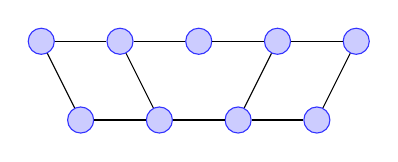
\begin{tikzpicture}
				\foreach \x in {1,...,5} {
					\node[vertex] (\x) at (\x,0) {};
				}
				\foreach \x [count = \i] in {6,...,9} {
					\node[vertex] (\x) at (\i.5,-1) {};
				}
				\foreach \x [evaluate=\x as \xplusone using int(\x + 1)] in {1,...,4,6,7,8} {
					\draw (\x) -- (\xplusone);
				}
				\draw (1) -- (6);
				\draw (5) -- (9);
				\draw (2) -- (7);
				\draw (4) -- (8);
			\end{tikzpicture}
		\end{figure}

		\item[(f)]
		The sequence (1, 2, 3, 4, 4, 5) cannot represent the degrees of the vertices in an undirected graph, since the sum of the sequence is 19, but the sum of the degrees of an undirected graph must always be even, since we have the following equation.
		\[\sum_{v \in V}\text{degree}(v) = 2|E|\]
	\end{enumerate}

	\bigskip
	\item[3.]
	Let \(G = (V, E)\) be an undirected, disconnected graph, and \(\overline{G} = (V, \overline{E})\) be its converse. Since it is disconnected, there must be more than one connected component. Let \(C\) be the set of all vertices in one such connected component, and \(D\) be the set of all vertices in all the other connected components. It follows that \(C \cup D = V\).

	Now, let \(c\) be any vertex in \(C\), and let \(d\) be any vertex in \(D\). Since \(c\) and \(d\) are in different connected components, the edge \((c, d) \notin E\). Therefore \((c, d) \in \overline{E}\). More simply put, every vertex in \(C\) is adjacent to every vertex in \(D\) in the graph \(\overline{G}\) and vice versa.

	Let us choose any specific vertex \(c_1 \in C\). We have just shown that \(c_1\) must be adjacent to every vertex in \(D\) in the graph \(\overline{G}\). So every vertex in \(D\), as well as the vertex \(c_1\) must be in the same connected component in \(\overline{G}\). Let us name this connected component \(A\).
	
	Now we shall choose a specific vertex \(d_1 \in D\). Similarly to the way \(c_1\) is adjacent to every vertex in \(D\), \(d_1\) must be adjacent to every vertex in \(C\). Therefore every vertex in \(C\) must be in the same connected component as \(d_1\), in the graph \(\overline{G}\).

	But we already established that \(d_1\) is in the connected component \(A\) since it is a vertex in \(D\), so every vertex in \(C\) must also be in the connected component \(A\). Now, since every vertex in \(C\) as well as every vertex in \(D\) is in the same connected component, therefore every vertex in \(V\) is in the same connected component --- since \(C \cup D = V\) --- in the graph \(\overline{G}\).

	Hence there is only one connected component in \(\overline{G}\), namely \(A\), so \(\overline{G}\) is connected.

	\bigskip
	\item[4.]
	Let \(G = (V, E)\) be an undirected connected graph, and let \(S \subset V\) be \textbf{non-empty}. Since \(G\) is connected, there must be a path between every two vertices in \(V\).

	Let \(a \in S\) and \(b \notin S\) be two vertices, and let \(P = (a, p_2, p_3, \dots, p_{n-1}, b)\) be a path between the two, where \(p_i\) is the \(i\)\textsuperscript{th} vertex in the path. There must be two consecutive vertices \(p_k\) and \(p_{k+1}\) such that \(p_k \in S\) and \(p_{k+1} \notin S\). To prove this claim, we will demonstrate a procedure to find \(k\).

	Begin at the vertices \(p_0\) and \(p_1\). We know that \(p_0 = a \in S\). Then we can check if the next vertex, \(p_1\) is in \(S\) or not. If \(p_1 \notin S\), then we have found that \(k = 0\). Otherwise, we know \(p_1 \in S\), and we may continue to the next step.

	Repeat the same process for the vertices \(p_1\) and \(p_2\), then for \(p_2\) and \(p_3\), \(p_3\) and \(p_4\), etc. until the vertices \(p_{n-2}\) and \(p_{n-1}\) are reached. One of two outcomes will have been reached thus far. Either we have found an \(i\) such that \(p_i \in S\) and \(p_{i+1} \notin S\), in which case \(k = i\); or we have not found such a number \(i\), in which case we know that \(p_0\) through \(p_{n-1}\) are all in \(S\). In case of the latter, we have \(p_{n-1} \in S\), but we know that \(p_n = b \notin S\). Therefore we have found that \(k = n - 1\).

	Since this procedure will always produce a \(k\) such that \(p_k \in S\) and \(p_{k+1} \notin S\), and every two consecutive vertices in a path --- which \(p_k \in S\) and \(p_{k+1}\) are --- must be adjacent, therefore we have a vertex which is not a member of \(S\) but has a neighbour which is.

	\bigskip
	\item[5.]
	\begin{enumerate}
		\item % a
		Given a set \(X = \{0, 1, 2, 3, 4\}\), where each subset of \(A \subset X\) such that \(|A| = 2\) is a vertex of a Petersen graph, there are \(\comb{5}{2}\) such subsets, so there are 10 vertices in a Petersen graph.

		\item % b
		Each vertex is a set with two elements, therefore there are three other elements which are not in each vertex. There are \(\comb{3}{2} = 3\) distinct sets of two elements that can be built from those three disjoint elements, so each vertex has a degree of three. The sum of all the degrees is thirty, and she sum of all the degrees bust be twice the number of edges, therefore there must be fifteen edges.

		\item % c
		As shown in part (b), there are three elements which are not in each vertex, of which \(\comb{3}{2}\) sets with a cardinality of two can be made. So each vertex is adjacent to three other vertices, so the degree of each vertex is three.

		\item % d
		We know a tree must be acyclic, but we will show that a Petersen graph has a cycle.
		
		Define a relation \(\to\) on two vertices in a Petersen graph as ``is adjacent to''. Using this relation, in a Petersen graph we have:
		\[\{0, 1\} \to \{2, 3\} \to \{0, 4\} \to \{1, 2\} \to \{3, 4\} \to \{0, 1\}\]

		This is a sequence of adjacent vertices, id est, a path, which has no immediate repetitions and begins and ends with the same node; hence a cycle. Therefore a Petersen graph is not a tree.
	\end{enumerate}

	\bigskip
	\item[6.]
	In a directed graph with no loops, each vertex can have an edge from itself to any vertex other than itself. Furthermore, unlike in an undirected graph, the existence of an edge from vertex \(\alpha\) to vertex \(\beta\) is independent of that of an edge from \(\beta\) to \(\alpha\).

	If there are \(n\) vertices in this directed graph and this graph has the maximal number of edges, then each of the \(n\) vertices has \(n - 1\) edges originating from it. Therefore the total number of edges in this graph is \(n(n - 1)\).

\end{enumerate}
    
\end{document}
